% Pipeline figure for the APS360 proposal.
% Compile on its own:  pdflatex pipeline.tex   ->  pipeline.pdf
\documentclass[tikz,border=2pt]{standalone}
\usepackage{times}
\usepackage{amsmath}
\usetikzlibrary{positioning,arrows.meta,fit,backgrounds,calc}

\definecolor{audio}{HTML}{2A6F97}
\definecolor{text}{HTML}{B5651D}
\definecolor{fuse}{HTML}{3B7D4F}
\definecolor{data}{HTML}{5E5E5E}
\definecolor{frozen}{HTML}{8C8C8C}

\begin{document}
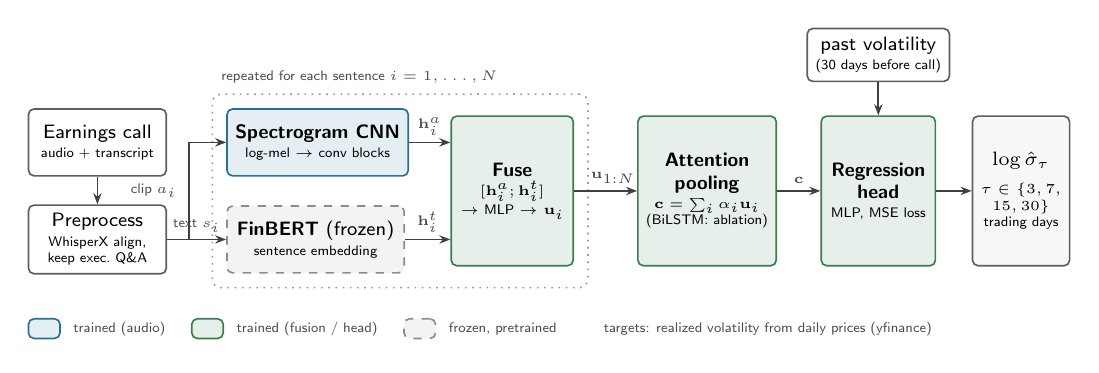
\begin{tikzpicture}[
    font=\sffamily\scriptsize,
    >={Stealth[length=4pt]},
    box/.style={draw, rounded corners=2pt, align=center, inner sep=3pt,
                minimum height=0.85cm, line width=0.6pt},
    train/.style={box, fill=#1!12, draw=#1},
    froz/.style={box, fill=frozen!10, draw=frozen, dashed},
    io/.style={box, fill=white, draw=data},
    arr/.style={->, line width=0.6pt, draw=black!75},
    lab/.style={font=\sffamily\tiny, text=black!70, align=center},
  ]

  % ---------------- inputs + preprocessing ----------------
  \node[io, minimum width=1.75cm] (call) {Earnings call\\[-1pt]\tiny audio + transcript};
  \node[io, below=0.35cm of call, minimum width=1.75cm] (prep)
       {Preprocess\\[-1pt]\tiny WhisperX align,\\[-2pt]\tiny keep exec.\ Q\&A};
  \draw[arr] (call) -- (prep);

  % ---------------- per-sentence branches ----------------
  \node[train=audio, right=0.75cm of call, minimum width=2.25cm] (cnn)
       {\textbf{Spectrogram CNN}\\[-1pt]\tiny log-mel $\rightarrow$ conv blocks};
  \node[froz, right=0.75cm of prep, minimum width=2.25cm] (bert)
       {\textbf{FinBERT} (frozen)\\[-1pt]\tiny sentence embedding};

  \draw[arr] (prep.east) -- ++(0.28,0) |- node[lab, pos=0.25, left=1pt] {clip $a_i$} (cnn.west);
  \draw[arr] (prep.east) -- node[lab, above=-1pt] {text $s_i$} (bert.west);

  \node[train=fuse, right=0.55cm of $(cnn.east)!0.5!(bert.east)$, minimum width=1.55cm,
        minimum height=1.9cm] (fuse)
       {\textbf{Fuse}\\[-1pt]\tiny $[\mathbf{h}^a_i;\mathbf{h}^t_i]$\\[-1pt]\tiny $\rightarrow$ MLP $\rightarrow \mathbf{u}_i$};
  \draw[arr] (cnn.east) -- node[lab, above=-1pt] {$\mathbf{h}^a_i$} (cnn.east -| fuse.west);
  \draw[arr] (bert.east) -- node[lab, above=-1pt] {$\mathbf{h}^t_i$} (bert.east -| fuse.west);

  % "for every sentence i" frame
  \begin{scope}[on background layer]
    \node[draw=black!40, dotted, rounded corners=3pt, line width=0.6pt,
          fit=(cnn)(bert)(fuse), inner sep=5pt,
          label={[lab, anchor=south west]north west:repeated for each sentence $i = 1,\dots,N$}] (rep) {};
  \end{scope}

  % ---------------- call-level ----------------
  \node[train=fuse, right=0.8cm of fuse, minimum width=1.6cm, minimum height=1.9cm] (pool)
       {\textbf{Attention}\\\textbf{pooling}\\[-1pt]\tiny $\mathbf{c}=\sum_i \alpha_i \mathbf{u}_i$\\[-2pt]\tiny (BiLSTM: ablation)};
  \draw[arr] (fuse) -- node[lab, above=-1pt, pos=0.62] {$\mathbf{u}_{1:N}$} (pool);

  \node[train=fuse, right=0.55cm of pool, minimum width=1.45cm, minimum height=1.9cm] (head)
       {\textbf{Regression}\\\textbf{head}\\[-1pt]\tiny MLP, MSE loss};
  \draw[arr] (pool) -- node[lab, above=-1pt] {$\mathbf{c}$} (head);

  \node[io, above=0.42cm of head, minimum width=1.45cm, minimum height=0.6cm] (pv)
       {past volatility\\[-1pt]\tiny (30 days before call)};
  \draw[arr] (pv) -- (head);

  \node[io, right=0.45cm of head, minimum width=1.2cm, minimum height=1.9cm, fill=fuse!5] (out)
       {$\log\hat{\sigma}_{\tau}$\\[2pt]\tiny $\tau\in\{3,7,$\\[-2pt]\tiny $15,30\}$\\[-2pt]\tiny trading days};
  \draw[arr] (head) -- (out);

  % ---------------- legend ----------------
  \node[train=audio, minimum height=0.25cm, minimum width=0.4cm, inner sep=0pt,
        below=0.55cm of prep.south west, anchor=north west] (l1) {};
  \node[lab, right=1pt of l1, anchor=west] (t1) {trained (audio)};
  \node[train=fuse, minimum height=0.25cm, minimum width=0.4cm, inner sep=0pt,
        right=0.2cm of t1] (l2) {};
  \node[lab, right=1pt of l2, anchor=west] (t2) {trained (fusion / head)};
  \node[froz, minimum height=0.25cm, minimum width=0.4cm, inner sep=0pt,
        right=0.2cm of t2] (l3) {};
  \node[lab, right=1pt of l3, anchor=west] (t3) {frozen, pretrained};
  \node[lab, right=0.35cm of t3, anchor=west]
       {targets: realized volatility from daily prices (yfinance)};
\end{tikzpicture}
\end{document}
